\subsection{Radioattività naturale}
Parte tutto dalle osservazioni di Bequerel della presenza di trasmutazioni di atomi. 
%IMMAGINE efr
\begin{figure}[htp!]
  \centering
  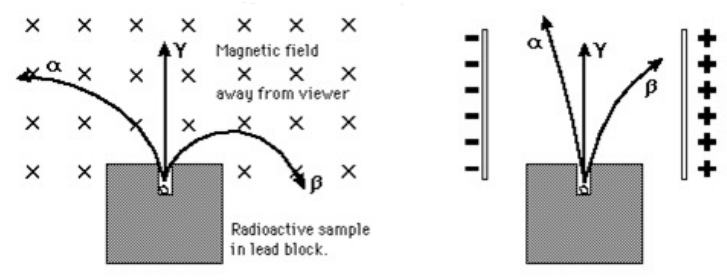
\includegraphics[scale=0.6]{Lezione3/efr.png} 
\end{figure}
Le radiazioni che vengono osservate hanno un'energia dell'ordine del $MeV$ di differenze carica e grado di penetrazione:
\begin{itemize}
    \item $\alpha$, nuclei di elio-4 ($\ch{^4He}$), $m=3726\,MeV$, $Q=+2$, $p\sim200\,MeV$;
    \item $\beta$, elettroni, $m=0.511\, MeV$, $Q=-1$, $p\sim1\,MeV$;
    \item $\gamma$, fotoni, $m=0\,MeV$, $Q=0$, $p\sim 1\,MeV$.
\end{itemize}
Genericamente i fenomeni di cui parliamo sono fenomeni spontanei che posso spiegare in termini di transizioni tra una struttura nucleare meno legata ad una più legata, con rilascio di energia. Studieremo alcune caratteristiche generali di questo processo:
\begin{itemize}
    \item condizioni perchè possa avvenire spontaneamente: \textbf{Q-valore};
    \item \textbf{ripartizione dell'energia} tra i prodotti di decadimento;
    \item \textbf{equazioni differenziali} che descrivono la radioattività;
    \item \textbf{condizione di equilibrio secolare} per catene di decadimenti
\end{itemize}
\subsection{Energia di disintegrazione (Q-value)}
Consideriamo un nucleo padre \textbf{P} che decade in due frammenti \textbf{D1} e \textbf{D2}. Per la conservazione dell'energia (se il nucleo padre è fermo la sua energia dipende dalla sua massa):
\begin{equation*}
    M_P=M_{D1}+T_{D1}+M_{D2}+T_{D2}
\end{equation*}
Dove $T_{D1}$ e $T_{D2}$ sono le energie cinetiche dei prodotti del decadimento. Definiamo energia di disintegrazione $Q$ come la differenza tra le masse del nucleo padre e dei frammenti:
\begin{equation*}
    Q=M_P-M_{D1}-M_{D2}
\end{equation*}
Di conseguenza \textbf{Q è l'energia a disposizione come energia cinetica dei frammenti}. Perchè il decadimento sia possibile $Q>0$. Per il decadimento $\alpha$:
\begin{equation*}
   \alpha: \qquad Q=M(A,Z)-M(A-4,Z-2)-M_\alpha
\end{equation*}
Per il decadimento $\beta$:
\begin{equation*}
    \beta^-: \qquad Q=M(A,Z)-M(A,Z+1)-M_e
\end{equation*}
\begin{equation*}
    \beta^+: \qquad Q=M(A,Z)-M(A,Z-1)-M_e
\end{equation*}
C'è un altro decadimento detto cattura elettronica in cui un nucleo cattura un elettrone e in questo processo di cattura libera energia. \textbf{E.C.}:
\begin{equation*}
    \textbf{E.C.}: \qquad Q=M(A,Z)+m_e-M(A,Z-1)
\end{equation*}
Da notare che si sta parlando di masse nucleari. Si possono trasformare in masse atomiche.
\subsection{Energia cinetica in decadimenti radioattivi}
\subsubsection{Versione non-relativistica}
Consideriamo il decadimento di \textbf{P} in quiete, per semplicità usiamo un decadimento $P\to D+\alpha$, ma le stesse considerazioni valgono per i decadimenti $\beta$. Essendo la particella padre in quiete e per il fatto che la quantità di moto si conserva avrò che anche la quantità di moto finale deve essere nulla. Essendo solo due i nuclei figli allora avrò che sono orientati in direzione opposa ma con lo stesso modulo. Un'altra condizione che imponiamo è la conservazione di energia cinetica:
\begin{equation*}
    p_\alpha=p_D \qquad T_\alpha+T_D=Q
\end{equation*}
Esprimendo il comune momento in termine di $T$:
\begin{equation*}
    2m_DT_D=2m_\alpha T_\alpha \quad \text{ in quanto: } p^2=2mT
\end{equation*}
Che possiamo riscrivere:
\begin{equation*}
    \frac{T_D}{T_\alpha}=\frac{m_\alpha}{m_D}
\end{equation*}
Il rapporto delle energie cinetiche è inversamentente proporzionale al rapporto delle masse: cioè più il frammento è leggero maggiore è l'energia cinetica che si forma.
\begin{equation*}
    T_\alpha=Q\frac{m_D}{m_D+m_\alpha} \qquad T_D=Q\frac{m_\alpha}{m_D+m_\alpha}
\end{equation*}
\textbf{Poichè $m\alpha\ll m_D$ il nucleo si porta una frazione piccola di $Q$}: ordine del $10^{-2}$ per decadimenti $\alpha$, ordine del $10^{-4}-10^{-5}$ per decadimenti $\beta/\gamma$.
\subsection{Legge dei decadimenti radioattivi}
Il tasso di decadimenti in un campione è una proprietà estensiva (proporzionale alla massa del campione):
\begin{equation*}
    -\frac{dN}{dt}=\lambda N
\end{equation*}
dove $N$ è  il numero di atomi nel campione, $\lambda$ è la \textbf{costante di decadimento} ed ha come unità di misura l'inverso del tempo. Quindi come definizione abbiamo che è la \textbf{probabilità di decadimento per unità di tempo}. Infatti la probabilità è una quantità adimensionale. Mentre $\lambda$ non lo è. Risolvendo l'equazione differenziale di ottiene l'andamento del numero di nuclei nel campione che ha un andamento esponenziale:
\begin{equation*}
    N(t)=N_0e^{-\lambda t}
\end{equation*}
\textbf{La vita media} di un atomo invece è data da:
\begin{equation*}
    \tau=\frac{1}{\lambda}
\end{equation*}
Che è uguale al tempo in cui il campione di nuclei si riduce di un fattore $e$. Un'altra quantità importante è il \textbf{tempo di dimezzamento}:
\begin{equation*}
    \tau_{1/2}=\tau\ln(2)
\end{equation*}
Si definisce \textbf{attività} di una sorgente il numero di decadimenti per unità di tempo. L'unità di misura è il \textbf{Bequerel}:
\begin{equation*}
    1\,Bq=1\,\text{decadimento}/s
\end{equation*}
storicamente è usato il \textbf{Curie} che è definito come attività di $1\,g$ di $\ch{^{226}Ra}$
\begin{equation*}
    1\,Ci=3.7\times10^{10}\,Bq
\end{equation*}
Un'altra definizione importante è la \textbf{larghezza di decadimento} che non è altro che la probabilità di decadimento per unità di tempo convertita in un'energia. Infatti abbiamo che $\hbar$ ha le dimensioni di un'energia per un tempo, quindi:
\begin{equation*}
    \Gamma=\hbar\lambda
\end{equation*}
Ad uno stato instabile si può associare un'incertezza sull'energia:
\begin{equation*}
    \Delta E\Delta t=\hbar \qquad \Delta E=\frac{\hbar}{\tau}=\Gamma
\end{equation*}
\subsection{Equilibrio nucleare}
In molti casi ci possiamo trovare di fronte ad un aumento del numero di atomi radioattivi, infatti oltre al decadimento radioattivo dei nuclei ci può esere anche un processo di produzione. Ad esempio la produzione per interazioni nucleare con raggi cosmici. La parte alta dell'atmosfera è bombardata continuamente da particelle accellerate da sorgenti astrofisiche e queste interazioni producono reazioni nucleari nell'atmosfera. 
\begin{equation*}
    \text{produzione }\ch{^{14}C}\, \text{ nei raggi cosmici }\, n+\ch{^{14}N}\to\ch{^{14}C}+p
\end{equation*}
Oppure la dalla produzione di radioisotopi ad accelleratori o reattori:
\begin{equation*}
    n+\ch{^{130}Tl}\to\ch{^{131}Tl}\to\ch{^{131}I}+\beta^{-}
\end{equation*}
Tasso di produzione: $R=\Phi N_{tg}\sigma$. Un altro caso in cui abbiamo processo di nuclei radioattivi è il caso di decadimenti a catena: ho un elemento radioattivo che decade in un altro elemento radioattivo e così via fino a quando non si trasmuta in un nucleo stabile. In tal caso l'evoluzione della popolazione segue una legge del tipo:
\begin{equation*}
    \frac{dN}{dt}=R-\lambda N
\end{equation*}
\textbf{Presenta una soluzione di equilibrio:} $N=R/\lambda$.
\begin{equation*}
    N(t)=\frac{R}{\lambda}+(N_0-\frac{R}{\lambda})e^{-\lambda t}
\end{equation*}
Questa soluzione ha un valore asintotico che è assunto dalla soluzione di equilibrio.
\subsection{Equazione secolare}
Consideriamo il caso di due sostanze radioattive:
\begin{equation*}
    S_1\to S_2\to S_3
\end{equation*}
La sostanza $S_1$ decade con la legge già vista, la quantità di sostanza $S_2$ invece aumenta quando $S_1$ diminuisce e diminuisce con la propria legge di decadimento. La sostanza $S_3$ è stabile e pertanto aumenta con il minuire di $S_2$:
\begin{equation*}
    \begin{dcases} \dfrac{dN_1}{dt}=-\lambda_1 N_1\\
\dfrac{dN_2}{dt}=\lambda_1N_1-\lambda_2N_2\\
\dfrac{dN_3}{dt}=\lambda_2N_2\\
\end{dcases}
\end{equation*}
Per $N_1$ si trova ovviamente la soluzione che avevamo trovato nel caso di una singola sostanza:
\begin{equation*}
    N_1(t)=N_{01}e^{-\lambda_1t}
\end{equation*}
Per $N_2$ scrivo la soluzione come:
\begin{equation*}
    N_2(t)=A_{21}e^{-\lambda_1t}+A_{22}+e^{-\lambda_2t}
\end{equation*}
La condizione iniziale per $N_2$ dà $A_{21}+A_{22}=N_{02}$ e dopo un po' di conti si arriva \textbf{all'equazione secolare}
\begin{equation*}
    N_2(t)=\frac{\lambda_1}{\lambda_2-\lambda_1}N_{01}(e^{-\lambda_1t}-e^{-\lambda_2t})+N_{02}e^{-\lambda_2t}
\end{equation*}
Un caso particolarmente interessante si ha quando le costanti di decadimento delle due sostanza sono molto diverse: un caso banale è quando $\lambda_2\ll\lambda_1$ e quindi $\tau_2\gg\tau_1$ e quindi l'elemento $1$ decade molto più velocemente dell'elemento $2$. E quindi succede che $S_1$ decade, si accumula in $S_2$ e successivamente con la sua legge di decadimento decate in $S_3$. Molto più interessante è il caso opposto: $\lambda_2\gg\lambda_1$ ($\tau_1\gg\tau_2$) e quindi si giunge "rapidamente" alla condizione $e^{-\lambda_2t}\sim 0$ e quindi rimane solo il termine:
\begin{equation*}
    N_2(t)\approx\frac{\lambda_1}{\lambda_2}N_{01}e^{-\lambda_1t}
\end{equation*}
Vediamo pertanto che per tempi $t\gg\tau_2=1/\lambda_2$ l'attività della sostanza $2$ segue la stessa evoluzione temporale della sostanza $1$. Per la sostanza $3$ basta integrare.
\subsection{Equilibrio secolare}
Se estendiamo questo ragionamento ad una catena più lunga, l'equazione differenziale diventa un po' più complicata:
\begin{equation*}
    N_1\to N_2\to N_3\to N_4\to \ldots
\end{equation*}
Se $\lambda_1\ll\lambda_i$ si instaura una condizione di equilibrio:
\begin{equation*}
    \lambda_1N_1=\lambda_2N_2=\lambda_3N_3= \ldots
\end{equation*}
Le attività degli anelli della catena sono uguali, quindi la popolazione è proporzionale alle vite medie.
\subsection{Radioattività naturale}
La radioattività naturale è dovuta a nuclei con vite medie dell'ordine della vita del sistema solare $\sim 4.5\times10^{9}\,yr$, e quindi tutti gli elementi che avevano una vita media minore in qualche modo sono quasi tutti decaduti e quello che ci rimane sono atomi che hanno una vita media maggiore. Queste avvengono tramite catene di $\alpha$ e $\beta$. Una volta che avviene un decadimento $\alpha$ ho una variazione di numero atomico $\Delta A =4$ e mi ritrovo nuclei ricchi di neutroni che decadono $\beta$.
\begin{itemize}
    \item $A=4n$, $\;\ch{^{232}Th}$, $\tau_{1/2}=1.39\times10^{10}\,yr$ $\to\ch{^{208}Pb}$
    \item $A=4n+1$, $\;\ch{^{237}Np}$, $\tau_{1/2}=2.2\times10^{6}\,yr$ $\to\ch{^{208}Bi}$
    \item $A=4n+2$, $\;\ch{^{238}U}$, $\tau_{1/2}=4.5\times10^{9}\,yr$  $\to\ch{^{206}Pb}$
    \item $A=4n+3$, $\;\ch{^{235}U}$, $\tau_{1/2}=7.15\times10^{8}\,yr$ $\to\ch{^{207}Pb}$
\end{itemize}
Un altro nucleo importante a lunga vita media è:
\begin{itemize}
    \item $\ch{^{40}K}\to\ch{^{40}Ca}+\beta^-$, $\tau_{1/2}=1.3\times10^{9}\,yr$
\end{itemize}
%IMMAGINE efr
\begin{figure}[htp!]
  \centering
  
\includegraphics[scale=0.5]{Lezione3/hh.png} 
\end{figure}
\subsection{Rapporti di decadimento}
Ci sono casi in cui un nucleo ha diversi processi di decadimento in competizione, ad esempio nella catena $4n$, il $\ch{^{212}Bi}$ decade con un tempo di dimezzamento di $61\, min$, nel $64\%$ dei casi $\beta$ in $\ch{^{212}Po}$ e nel $36\%$ dei casi $\alpha$ in $\ch{^{208}Tl}$. Il processo è caratterizzato dalle \textbf{probabilità di decadimento per unità di tempo} $\lambda_i$ in ogni canale possibile. Il nucleo padre segue una legge esponenziale \textbf{costante di decadimento}: $\lambda=\sum_i\lambda_i$. Il \textbf{rapporto di decadimento}, o \textbf{branching ratio}, in un certo canale è dato dalla frazione di decadimenti in quel canale:
\begin{equation*}
    \text{BR}_i=\frac{|dN_i/dt|}{|dN/dt|}=\frac{\lambda_i}{\lambda}
\end{equation*}
Si definiscono le \textbf{larghezze di decadimento totale e parziali}
\begin{equation*}
    \Gamma=\hbar\lambda \qquad \Gamma_i=\hbar\lambda_i
\end{equation*}
\subsection{Statistica di conteggio}
Nel trattamento fin quì fatto abbiamo considerato $N(t)$ una funzione continua dal momento che il numero di nuclei considerati è usualmente molto elevato l'approssimazione risulta adeguata. Per descrivere correttamente le fluttuazioni degli esperimenti di conteggio occorre tenere conto esplicitamente della natura discreta di $N$. Consideriamo $N$ nuclei radioattivi caratterizzati dalla costante di decadimento $\lambda$. In un intervatto $\Delta t$ la probabilità di decadimento di un nucleo particolare è $p=\lambda\Delta t$. La probabilità che $k$ nuclei qualsiasi decadano è data dalla \textbf{distribuzione binomiale}:
\begin{equation*}
    P(N,k)=\frac{N!}{k!(N-k)!}p^k(1-p)^{N-k}
\end{equation*}
Visto che i numeri con cui abbiamo a che fare sono molto grandi cerchiamo una formula approssimata per $P(N,k)$ nel caso in cui: $N\gg1$, $p\ll1$ e $k\sim pN\ll N$. Dato che $p\ll1$ possiamo scrivere:
\begin{equation*}
    \binom{N}{k}\approx\frac{N^k}{k!}
\end{equation*}
e
\begin{equation*}
    1-p\approx e^{-p} \quad (1-p)^{N-k}\approx(e^{-p})^{N-k}=e^{-Np+kp}\approx e^{Np}
\end{equation*}
Questo perchè $Np\sim k $, $p\ll1$ e $kp\ll Np$. Mettendo insieme i vari termini che sono stati approssimati ottengo:
\begin{equation*}
 P(N,k)=\frac{N^k}{k!}p^ke^{-Np}   
\end{equation*}
Se definiamo $\Bar{n}=pN$ che rappresenta il numero medio di decadimenti che osservo in un intervallo di tempo $\Delta t$ otteniamo la \textbf{distribuzione di Poisson}. 
\begin{equation*}
    P(\Bar{n},k)=\frac{\Bar{n}^k}{k!}e^{-\Bar{n}}
\end{equation*}
E' la probabilità di osservare $k$ decadimenti quando il numero di decadimenti è $\Bar{n}$. Consideriamo un nucleo con una costante di decadimento $\lambda$, misuriamo con un rivelatore il numero di decadimenti nell'intervallo $\Delta t$:
\begin{equation*}
    \Bar{n}=pN=N\lambda\Delta t
\end{equation*}
\subsection{Distribuzione temporale}
La formulazione che abbiamo appena visto è la stessa che si utilizza per descrivere la probabilità di registrare $k$ eventi distribuiti casualmente, con probabilità uniforme e in un intervallo temporale $\Delta t=t_2-t_1$. Se si hanno $N_{obs}$ eventi ossevati in un intervallo $0-T$ abbastanza lungo si può definire \textbf{l'attivita o tasso d decadimento}:
\begin{equation*}
    A=\frac{N_{obs}}{T}
\end{equation*}
E la probabilità che questi eventi cadano proprio in questo intervallo di tempo è:
\begin{equation*}
    p=\frac{t_2-t_1}{T}
\end{equation*}
Mentre gli eventi attesi:
\begin{equation*}
    \Bar{n}=pN_{obs}=A(t_2-t_1)
\end{equation*}
La probabilità di osservarne $k$ nell'intervallo $t_2-t_1$ segue la distribuzione di Poisson che abbiamo ricavato in precedenza. 

\textbf{Distribuzione temporale} è la probabilità di osservare un intervallo $t$ tra due decadimenti ed è data dalla probabilità di osservare $0$ decadimenti nell'intervallo temporale:
\begin{equation*}
    P(\Bar{n},0)=\frac{\Bar{n}^0}{0!}e^{-\Bar{n}}=e^{-\Bar{n}}
\end{equation*}
Dove $\Bar{n}$ può essere definita come $\Bar{n}=At$ e quindi:
\begin{equation*}
    P(t)dt=e^{-\Bar{n}(t)}(Adt)=e^{-At}Adt
\end{equation*}
\subsection{Esempio: datazione con carbonio-14}
Il $\ch{^{14}C}$ viene prodotto dai raggi cosmici: 
\begin{equation*}
    n+\ch{^{14}N}\to\ch{^{14}C}+p
\end{equation*}
Si lega con l'ossigeno atmosferico per dare $\ch{CO_2}$ che viene metabolizzato dalla vegetazione e dagli animali che se ne nutrono. Il carbonio-14 decade beta
\begin{equation*}
    \ch{^{14}C}\to\ch{^{14}N}+\beta^- \qquad \tau_{1/2}=5700\,yr
\end{equation*}
All'equilibrio $1\,g$ di $C$ (carbonio naturale l'insieme di tutti gli isotopi) ha un'attività di $15$ decadimenti/minuto ($A_0=0.25\,Bq/g$). Il carbonio-14 esce da questo equilibrio una volta che l'organismo muore. In quanto quell'organismo non assorbe più carbonio. 

Supponiamo di misurare in una massa $m$ di $C$, $N$ decadimenti in un tempo $T$: \textbf{come stimiamo l'età del campione e con che incertezza?} Il valore dell'attività $A$ è dato da:
\begin{equation*}
    A(t)=\frac{N}{T}\pm\frac{\sqrt{N}}{T}
\end{equation*}
La dipendenza di $A(t)$ dal tempo è:
\begin{equation*}
   A(t)= mA_0e^{-\lambda t}
\end{equation*}
Da cui si ricava
\begin{equation*}
    t=-\frac{1}{\lambda}\ln{\frac{A(t)}{mA_0}}=-\frac{\tau_{1/2}}{\ln{2}}\ln{\frac{A(t)}{mA_0}}
\end{equation*}
L'incertezza:
\begin{equation*}
    \sigma_t=\left| \frac{d}{dA}(-\frac{1}{\lambda}\ln{\frac{A(t)}{mA_0}}) \right|\sigma_A=\frac{\tau_{1/2}}{\ln{2}}\frac{\sigma_A}{A(t)}=\frac{\tau_{1/2}}{\ln{2}}\frac{1}{\sqrt{N}}
\end{equation*}
Poichè $N(t)=A(t)T$, l'incertezza diminuisce con l'aumentare del tempo e 
\begin{equation*}
    \frac{\sigma_t}{t}=-\frac{1}{\sqrt{A(t)T}\ln{A(t)/mA_0}}=\frac{e^{\lambda t/2}}{\sqrt{mA_0T}\lambda t}
\end{equation*}
Questo ci porta a dare una certa condizione in cui una misura è efficace o no. Questo rapporto tende a infinito e quindi ad un valore grande e quindi non sono in grado di misurare in due casi: il primo è per tempi molto piccoli, infatti predomina il denominatore che per $t\to0$ mi manda il rapporto a infinito. Il secondo è per tempi molto grandi. Infatti per $t\to \infty$ il numeratore va come un'esponenziale e quindi mi manda il rapporto a infinito. Questo significa che quando ormai tutto il carbonio è decaduto non ho più la sensibilità per fare una misura accurata dell'attività.